\documentclass[journal]{IEEEtran}
\usepackage{blindtext}
\usepackage{graphicx}

\usepackage[cmex10]{amsmath}
\usepackage{array}

\usepackage{float}

\usepackage{mdwmath}
\usepackage{mdwtab}

\usepackage{fixltx2e}

\usepackage{tikz}
\usetikzlibrary{
  arrows,
  shapes,
  trees,
  intersections,
  shadows,
  positioning,
  decorations.pathmorphing,
  fit,
  petri,
  backgrounds,
  calc
}

% for showing geometry details wrt pdf rendering
%\usepackage[showframe]{geometry}% http://ctan.org/pkg/geometry

% correct bad hyphenation here
\hyphenation{op-tical net-works semi-conduc-tor}

\begin{document}

% can use linebreaks \\ within to get better formatting as desired
\title{Investigating in-vitro neuron cultures as computational reservoir}

\author{Peter Aaser}
%
% make the title area
\maketitle

\begin{abstract}
  \blindtext[2]

\end{abstract}

\begin{IEEEkeywords}
memes, reddit, unfunny, low-energy
\end{IEEEkeywords}

\section{Introduction}
Since the 50s, the Von-Neumann computer architecture has been ubiquitous in the
field of computing. This architecture owes its success to its relative
simplicity, allowing quick iterations in tact with doubling transistor counts in
accord with moores law.
However several issues with the Von-Neumann architecture have become more and more
pressing in recent times. Issues such as the Von-Neumann memory bottleneck are
becoming increasingly difficult to hide, and its inherently serial nature of computation.
Even in the case that moores law will continue, we still face issues with lack
of scalability in modern processors.
With billions of transistors a top down
design process is becoming increasingly difficult and expensive, and a single
faulty transistor can cause an entire chip to be useless.
These weaknesses necessitates going beyond the Von-Neumann architecture,
exploring unconventional computing paradigms.
Taking inspiration from nature we
look at cellular computing consisting of computational cells which by themselves
are unremarkable.
In these systems we observe properties that cannot be
traced back to a single cell, they only appear when multiple cells are
interacting with each other.
In nature these systems form without any form of supervision, a property known
as \textit{self organization}, with an example being 
DNA which ``describes how to build the system, not what the system will look
like'' \cite{tufte_evo_2009}.
These \textit{emergent properties} arise in systems built from the bottom up by
%
a set of growth rules rather than a designers intent, a  property, which allows a flexibility and robustness that modern
processors lack, a prime example being the human brain.
%
The human brain is a vastly parallel computer, eclipsing modern processors in
terms of computational capacity, robustness, energy efficiency and complexity.
The three first properties make them very appealing subjects to study for
unconventional computing, however due to the immense complexity the brain is
still enigmatic.
In this paper we explore using neuron cultures to create an organic mechanical
hybrid organism, a so called \textit{cyborg}.

%%% Local Variables:
%%% mode: latex
%%% TeX-master: "../main"
%%% End:
\section{Background}
\subsection{The NTNU Cyborg Project}
The NTNU cyborg project is a collaboration between several departments at NTNU
including the department of biotechnology, computer and information science,
engineering cybernetics, neuroscience and more. \cite{fossen_ntnu_???}
The stated goal for the cyborg project is ``to enable communication between living
nerve tissue and a robot. The social and interactive cyborg will walk around the campus
raising awareness for biotechnology and ICT, bringing NTNU in the forefront of research
and creating a platform for interdisciplinary collaborations and teaching.''
Currently the department of neuroscience is growing neuron cultures which are to
be used as the biological part of the robot.
These neuron cultures are not part of a brain, they are fully dissociated, grown
in special chambers in-vitro.
The robot part of the cyborg has been developed and implemented by the
department of engineering cybernetics, and is currently operational, however it
has not yet been integrated with the in-vitro neuron cultures.
The challenge faced by the cyborg project is the infrastructure for interfacing the
neuron cultures and the robot, essentially creating a brain computer interface.
\subsection{Complex Systems}
\textit{
  In this paper references are made to computations done by both artificial and real
  neurons.
  To make the distinction between these cases clear all computation done by
  computer simulated approximations of neurons will be prefixed as artificial.
}\\
The self-organizing properties that makes cellular computing a such a successful
paradigm in nature also make understanding and exploiting them difficult.
Many such systems have been explored, such as recurrent artificial neural
networks \cite{bertschinger_real-time_2004}, random boolean networks
\cite{gershenson_introduction_2004} and cellular automata.
In \cite{langton_computation_1990} Langton explores the requirements for systems
to support emergent computation, where
he argues that in order for a system to support emergent computation it must
lie in a \textit{critical phase} between order and chaos, drawing parallels to
phase transitions in material science.
This observation comes from thermodynamics, in which a material may exhibit a
\textit{second order phase transition} between a solid and liquid form where the
material undergoes a continuous transition in contrast to a first order
transition such as melting ice.
Using cellular automata as an example, he explores the effect of varying the
rules for calculating the next state with a parameter, $\lambda$, which
describes how likely it is for a cell to enter a \textit{quiescent state}, a state
where it will not disturb other cells until it leaves the quiescent state itself.
At $\lambda = 0$ all cells enter a quiescent state after one step, representing
a fully ordered system, thus at $\lambda = 0$ the system is in the ordered phase.
At $\lambda = 1$ there are no rules that leads to a quiescent state, leading to
very chaotic systems with very high entropy, representing the chaotic phase.
As $\lambda$ is increased from 0 the cellular systems starts to form intricate
structures, increasing in complexity and taking longer to reach a steady state.
This behavior peaks at $\lambda \approx 0.5$ which is the most critical phase in this
particular system, creating complex self-organizing structures.
As $\lambda$ is increased further the self-organizing structures start to give
way to more chaotic and seemingly random behavior, gradually transitioning into
the chaotic phase.\\
It turns out then, that with most cellular systems providing the necessary
conditions for computation to occur is a tractable problem, however harnessing
and shaping this computation is a whole different matter.
In their critical phase systems are unstable but not chaotic which causes them to
be highly sensitive to small changes in topology and initial conditions.
Attempting to maneuver this fitness-landscape by directly changing the
properties of a system would in many ways be like calculating the correct way
for a butterfly in china to flap its wings in order to cause a hurricane in New York.\\
\subsection{Reservoir Computing}
Faced with the intractability of designing cellular computation systems in a top
down manner, and the unpredictable relation between cause and effect in self organizing
systems has made it necessary to approach complex systems in a different manner.
One such approach is to treat the system as a \textit{reservoir}
\cite{schrauwen_overview_2007} which
``acts as a complex nonlinear dynamic filter that transforms the
input signals using a high-dimensional temporal map, not unlike the operation
of an explicit, temporal kernel function.''\\
AAAAAA
\ref{fig:RC} shows a typical RC (reservoir computing) system with three inputs
and two outputs. The inputs are processed in a simple feed-forward neural
network before perturbing the reservoir in some way.
Similarly the state of the reservoir is being processed by an output layer
before leaving the RC system.
In the figure the input and output processing is done by feed forward neural
networks, but we note that this is only one of many possible filters.
Inputs 1, 2 and 3 are snapshots of the current state of the problem we attempt
to solve with reservoir computing.
Since our filters have no state, at least not beyond some time horizon we see
that the history of the system must in some way be encoded in the reservoir in
order for the RC system to solve problems in scope wider than the limited amount
of state that may be contained in the filters.
\begin{figure*}[h]
  % \begin{tikzpicture}[scale=3]
%   \clip (-2,-0.3) rectangle (2,0.9);
%   \draw[step=.5cm,gray,very thin] (-1.4,-1.4) grid (1.4,1.4);
%   \filldraw[fill=green!20,draw=green!50!black] (0,0) -- (3mm,0mm)
%     arc [start angle=0, end angle=30, radius=3mm] -- cycle;
% 
%   \draw[->] (-1.5,0) -- (1.5,0) coordinate (x axis);
%   \draw[->] (0,-1.5) -- (0,1.5) coordinate (y axis);
%   \draw (0,0) circle [radius=1cm];
%   \draw[very thick,red]
%     (30:1cm) -- node[left=1pt,fill=white] {$\sin \alpha$} (30:1cm |- x axis);
% 
%   \draw[very thick,blue]
%     (30:1cm |- x axis) -- node[below=2pt,fill=white] {$\cos \alpha$} (0,0);
% 
%   \path [name path=upward line] (1,0) -- (1,1);
%   \path [name path=sloped line] (0,0) -- (30:1.5cm);
%   \draw [name intersections={of=upward line and sloped line, by=t}]
%     [very thick,orange] (1,0) -- node [right=1pt,fill=white]
%     {$\displaystyle \tan \alpha \color{black}=
%       \frac{{\color{red}\sin \alpha}}{\color{blue}\cos \alpha}$} (t);
% 
%   \draw (0,0) -- (t);
%   \foreach \x/\xtext in {-1, -0.5/-\frac{1}{2}, 1}
%   \draw (\x cm,1pt) -- (\x cm,-1pt) node[anchor=north,fill=white] {$\xtext$};
%   \foreach \y/\ytext in {-1, -0.5/-\frac{1}{2}, 0.5/\frac{1}{2}, 1}
%   \draw (1pt,\y cm) -- (-1pt,\y cm) node[anchor=east,fill=white] {$\ytext$};
% \end{tikzpicture}
\pgfdeclarelayer{background}
\pgfdeclarelayer{foreground}
\pgfsetlayers{background,main,foreground}

% Define block styles used later
\tikzstyle{sensor}=[draw, fill=blue!20, text width=5em, 
    text centered, minimum height=2.5em,drop shadow]

\tikzstyle{ann} = [above, text width=5em, text centered]

\tikzstyle{wa} = [sensor, text width=10em, fill=red!20, 
    minimum height=6em, rounded corners, drop shadow]

\tikzstyle{sc} = [sensor, text width=13em, fill=red!20, 
    minimum height=10em, rounded corners, drop shadow]

% Define distances for bordering
\def\blockdist{2.3}
\def\edgedist{2.5}

\begin{figure}[p]
\begin{tikzpicture}
    \node (wa) [wa]  {System Combination};
    \path (wa.west)+(-3.2,1.5) node (asr1) [sensor] {$ASR_1$};
    \path (wa.west)+(-3.2,0.5) node (asr2) [sensor] {$ASR_2$};
    \path (wa.west)+(-3.2,-1.0) node (dots) [ann] {$\vdots$}; 
    \path (wa.west)+(-3.2,-2.0) node (asr3)[sensor] {$ASR_N$};    
   
    \path (wa.east)+(\blockdist,0) node (vote) [sensor] {$\theta_0,\theta_1,...,\theta_M$\\Estimated Parameters};

    \path [draw, ->] (asr1.east) -- node [above] {} 
        (wa.160) ;
    \path [draw, ->] (asr2.east) -- node [above] {} 
        (wa.180);
    \path [draw, ->] (asr3.east) -- node [above] {} 
        (wa.200);
    \path [draw, ->] (wa.east) -- node [above] {} 
        (vote.west);

               
    \path (wa.south) +(0,-\blockdist) node (asrs) {System Combination - Training};
  
    \begin{pgfonlayer}{background}
        \path (asr1.west |- asr1.north)+(-0.5,0.3) node (a) {};
        %\path (wa.south -| wa.east)+(+0.5,-0.3) node (b) {};
        \path (vote.east |- asrs.east)+(+0.5,-0.5) node (c) {};
          
        \path[fill=yellow!20,rounded corners, draw=black!50, dashed]
            (a) rectangle (c);           
        \path (asr1.north west)+(-0.2,0.2) node (a) {};
            
    \end{pgfonlayer}
    
    % Validation Layer is the same except that there are a set of nodes and links which are added
   

    % \path (wa.south)+(-2.0,-7.5) node (syscomb) [sc] {\textbf{System Combination \\Algorithm}\\Estimated Parameters\\from training};
    % \path (syscomb.west)+(-2.2,1.5) node (asrt1) [sensor] {$ASR_1$};
    % \path (syscomb.west)+(-2.2,0.5) node (asrt2)[sensor] {$ASR_2$};
    % \path (syscomb.west)+(-2.2,-1.0) node (dots)[ann] {$\vdots$}; 
    % \path (syscomb.west)+(-2.2,-2.0) node (asrt3)[sensor] {$ASR_N$};    

    % \path [draw, ->] (asrt1.east) -- node [above] {} 
    %     (syscomb.160) ;
    % \path [draw, ->] (asrt2.east) -- node [above] {} 
    %     (syscomb.180);
    % \path [draw, ->] (asrt3.east) -- node [above] {} 
    %     (syscomb.200);

    %            
    % \path (wa.south) +(0,-\blockdist) node (sct) {System Combination - Training};
 

    % \path (syscomb.east)+(1.0,0.0) node (bwtn) {};

    % % Note how the single nodes are repeated using for loop
    % \foreach \x in {0,1,...,4} 
    % { 
    %     \draw (bwtn.east)+(\x,0) node (asr\x-2)[]{}; 
    %     \fill (bwtn.east)+(\x,0) circle (0.1cm); 
    % }
   
    % \path [draw, ->] (syscomb.east) -- node [above] {} 
    %     (bwtn.east);
	  % \path [draw, ->] (asr0-2) -- node [above] {@} 
    %     (asr1-2);
    % \path [draw, -] (asr1-2) -- node [above] {b} 
    %     (asr2-2);
    % \path [draw, -] (asr2-2) -- node [above] {z} 
    %     (asr3-2);
    % \path [draw, -] (asr3-2) -- node [above] {} 
    %     (asr4-2);

    % \path [draw, ->] (asr0-2) edge[bend  right]  node [below] {@} 
    %     (asr1-2);
    % \path [draw, ->] (asr1-2) edge[bend  right]  node [below] {b} 
    %     (asr2-2);
    % \path [draw, ->] (asr2-2) edge[bend  right]  node [below] {c} 
    %     (asr3-2);
    % \path [draw, ->] (asr4-2) node[]{} (asr4-2)+(1.0,0);

    % \begin{scope}[looseness=1.6]
    %     \path [draw, ->] (asr0-2) edge[bend  right=90]  node [below] {a} 
    %         (asr1-2);
    %     \path [draw, ->] (asr1-2) edge[bend  right=90]  node [below] {b} 
    %         (asr2-2);
    %     \path [draw, ->] (asr2-2) edge[bend  right=90]  node [below] {c} 
    %         (asr3-2);
    % \end{scope}
    % \path (asr3-2.east)+(1.5,0.0) node (bw)[sensor] {Best Word Sequence\\$\arg\max$};    

    % \path [draw, -] (asr1-2.east) node [below] {} 
    %     (bw.west);
    %       
    % \begin{pgfonlayer}{background}
    %     \path (asrt1.west)+(-0.5,1.0) node (g) {};
    %     \path (bw.east |- syscomb.south)+(0.5,-1.5) node (h) {};
    %      
    %     \path[fill=yellow!20,rounded corners, draw=black!50, dashed]
    %         (g) rectangle (h);

    %     \path [draw, ->] (vote.south) edge[bend  left=90]  node [below] {Used in validation} 
    %         (syscomb.30);            

    % \end{pgfonlayer}
    % 
    % \path (asr1-2.south) +(-\blockdist,-\blockdist) 
    %     node (asrs) {System Combination - Validation};

  \end{tikzpicture}
\end{figure}
  \caption{A reservoir comput-thingy}
  \label{fig:RC}
\end{figure*}
\subsection{Neuron Computing}
The human brain consist of 100 billion neurons, forming a vastly complex
hierarchy of behavior, from the neuron-level interactions to the interaction
between different parts of the brain such as the hippocampus and the frontal lobe.
The basic building block of the brain is the neuron, which even by itself is a
very complex system, not at all analogous to a single transistor or an artificial
neuron.
These neurons communicate with each others using electric and chemical signals
in a complex interplay between neurotransmitters, voltage spikes and even
rearranging their physical structures, growing new connections and letting
unused connections wither.
The complexities of neurons have been widely studied, but for this paper a
cursory introduction is sufficient.
We will only consider a generalized version of the neuron, but in our
experiments a plethora of different neurons are used, although they
all share the basic similarities described here.
The anatomy of a neuron is shown in \ref{fig:neuron_anatomy} and can roughly be
divided into the following parts:
\subsubsection{Soma}
The main body of the neuron.
\subsubsection{Dendrites}
To sense its surroundings the neuron is equipped with dendrites. These
branching structures act as receivers, propagating electro-chemical stimuli to
the cell body. Their reach is only to the immediate vicinity of the cell, they
do not form longer connections.
\subsubsection{Axon}
The axon is a long tendril, extending over a meter in the case of the sciatic
nerve, which transmits information as electrical pulses to other neurons. An
axon can branch off and reach multiple neurons, it is not a one to one
connection.
\subsection{Adaptivity}
Write about evolvable systems. Possibly evo-devo?
Something in relation to understanding the underlying growth rules (devo) using
evolution, in contrast to directly evolving phenotypes.

\begin{figure*}[p]
    \centering
    \includegraphics[width=\textwidth]{images/"Neuron anatomy".png}
    \caption{a neuron}
    \label{fig:neuron_anatomy}
\end{figure*}

%%% Local Variables:
%%% mode: latex
%%% TeX-master: "../main"
%%% End:
\section{A Hybrid Neuro-Digital Approach}
\subsection{Concept}
A neural network is grown in a \textit{MEA}, short for \textit{micro electrode
 array} which allows the neurons to be interfaced with using electrical stimuli
in order to control a robot as shown in \ref{fig:cyborg_idea}.
Building on the theoretical groundwork described in the background, the neural
network is used as a reservoir which is fed sensory input from a robot.
This system is a \textit{closed loop}, it does not require any outside
intervention such as a human controller using a joystick to operate.
A somewhat subtle but very important consequence of utilizing reservoir
computing is that the neural network does not directly control the robot, it
simply acts as a classifier which responds to the input, and the resulting
dynamics is interpreted by a computer as an action for the robot.
This distinction has little practical consequence for the cyborg, but may offer
a clue into the inner workings of sentience.
\begin{figure}[h!]
    %\centering
    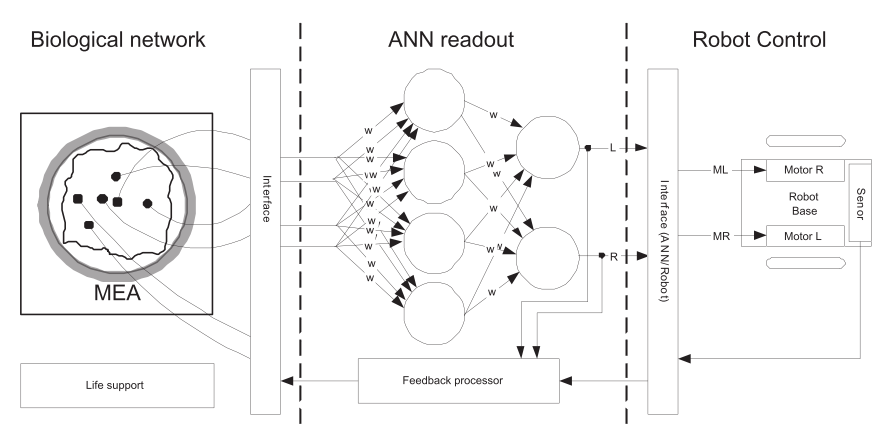
\includegraphics[width=\linewidth]{images/cyborg_overview.png}
    \caption{The gist of it..}
    \label{fig:cyborg_idea}
\end{figure}
\subsection{Platform}
Providing an interface between neurons and a computer allows using neural
network for computation, however it is impractical to move the neural cultures
outside of the laboratory.
The practical, yet thought provoking\footnote{For brevity the
  philosophical implications is left as an exercise to the reader.} solution is
using a TCP/IP network protocol such that the neuron culture may be interfaced with any
robot or simulator without leaving the laboratory.
Similar network architectures have been implemented, in
\cite{li_application_2015} a neuron culture is used to control a simple
wall-avoiding robot as a proof of concept.
In contrast with previous work the robot used in the NTNU cyborg project is a
sophisticated robot which can move by itself, follow a person, take a selfie
with someone and upload it to facebook, and even perform a secret handshake.
By utilizing an already functioning robot as a host the cyborg project can focus
on extending the capabilities of the robot, making it a true hybrid between
digital and cellular computing.
\begin{figure}[h!]
    %\centering
    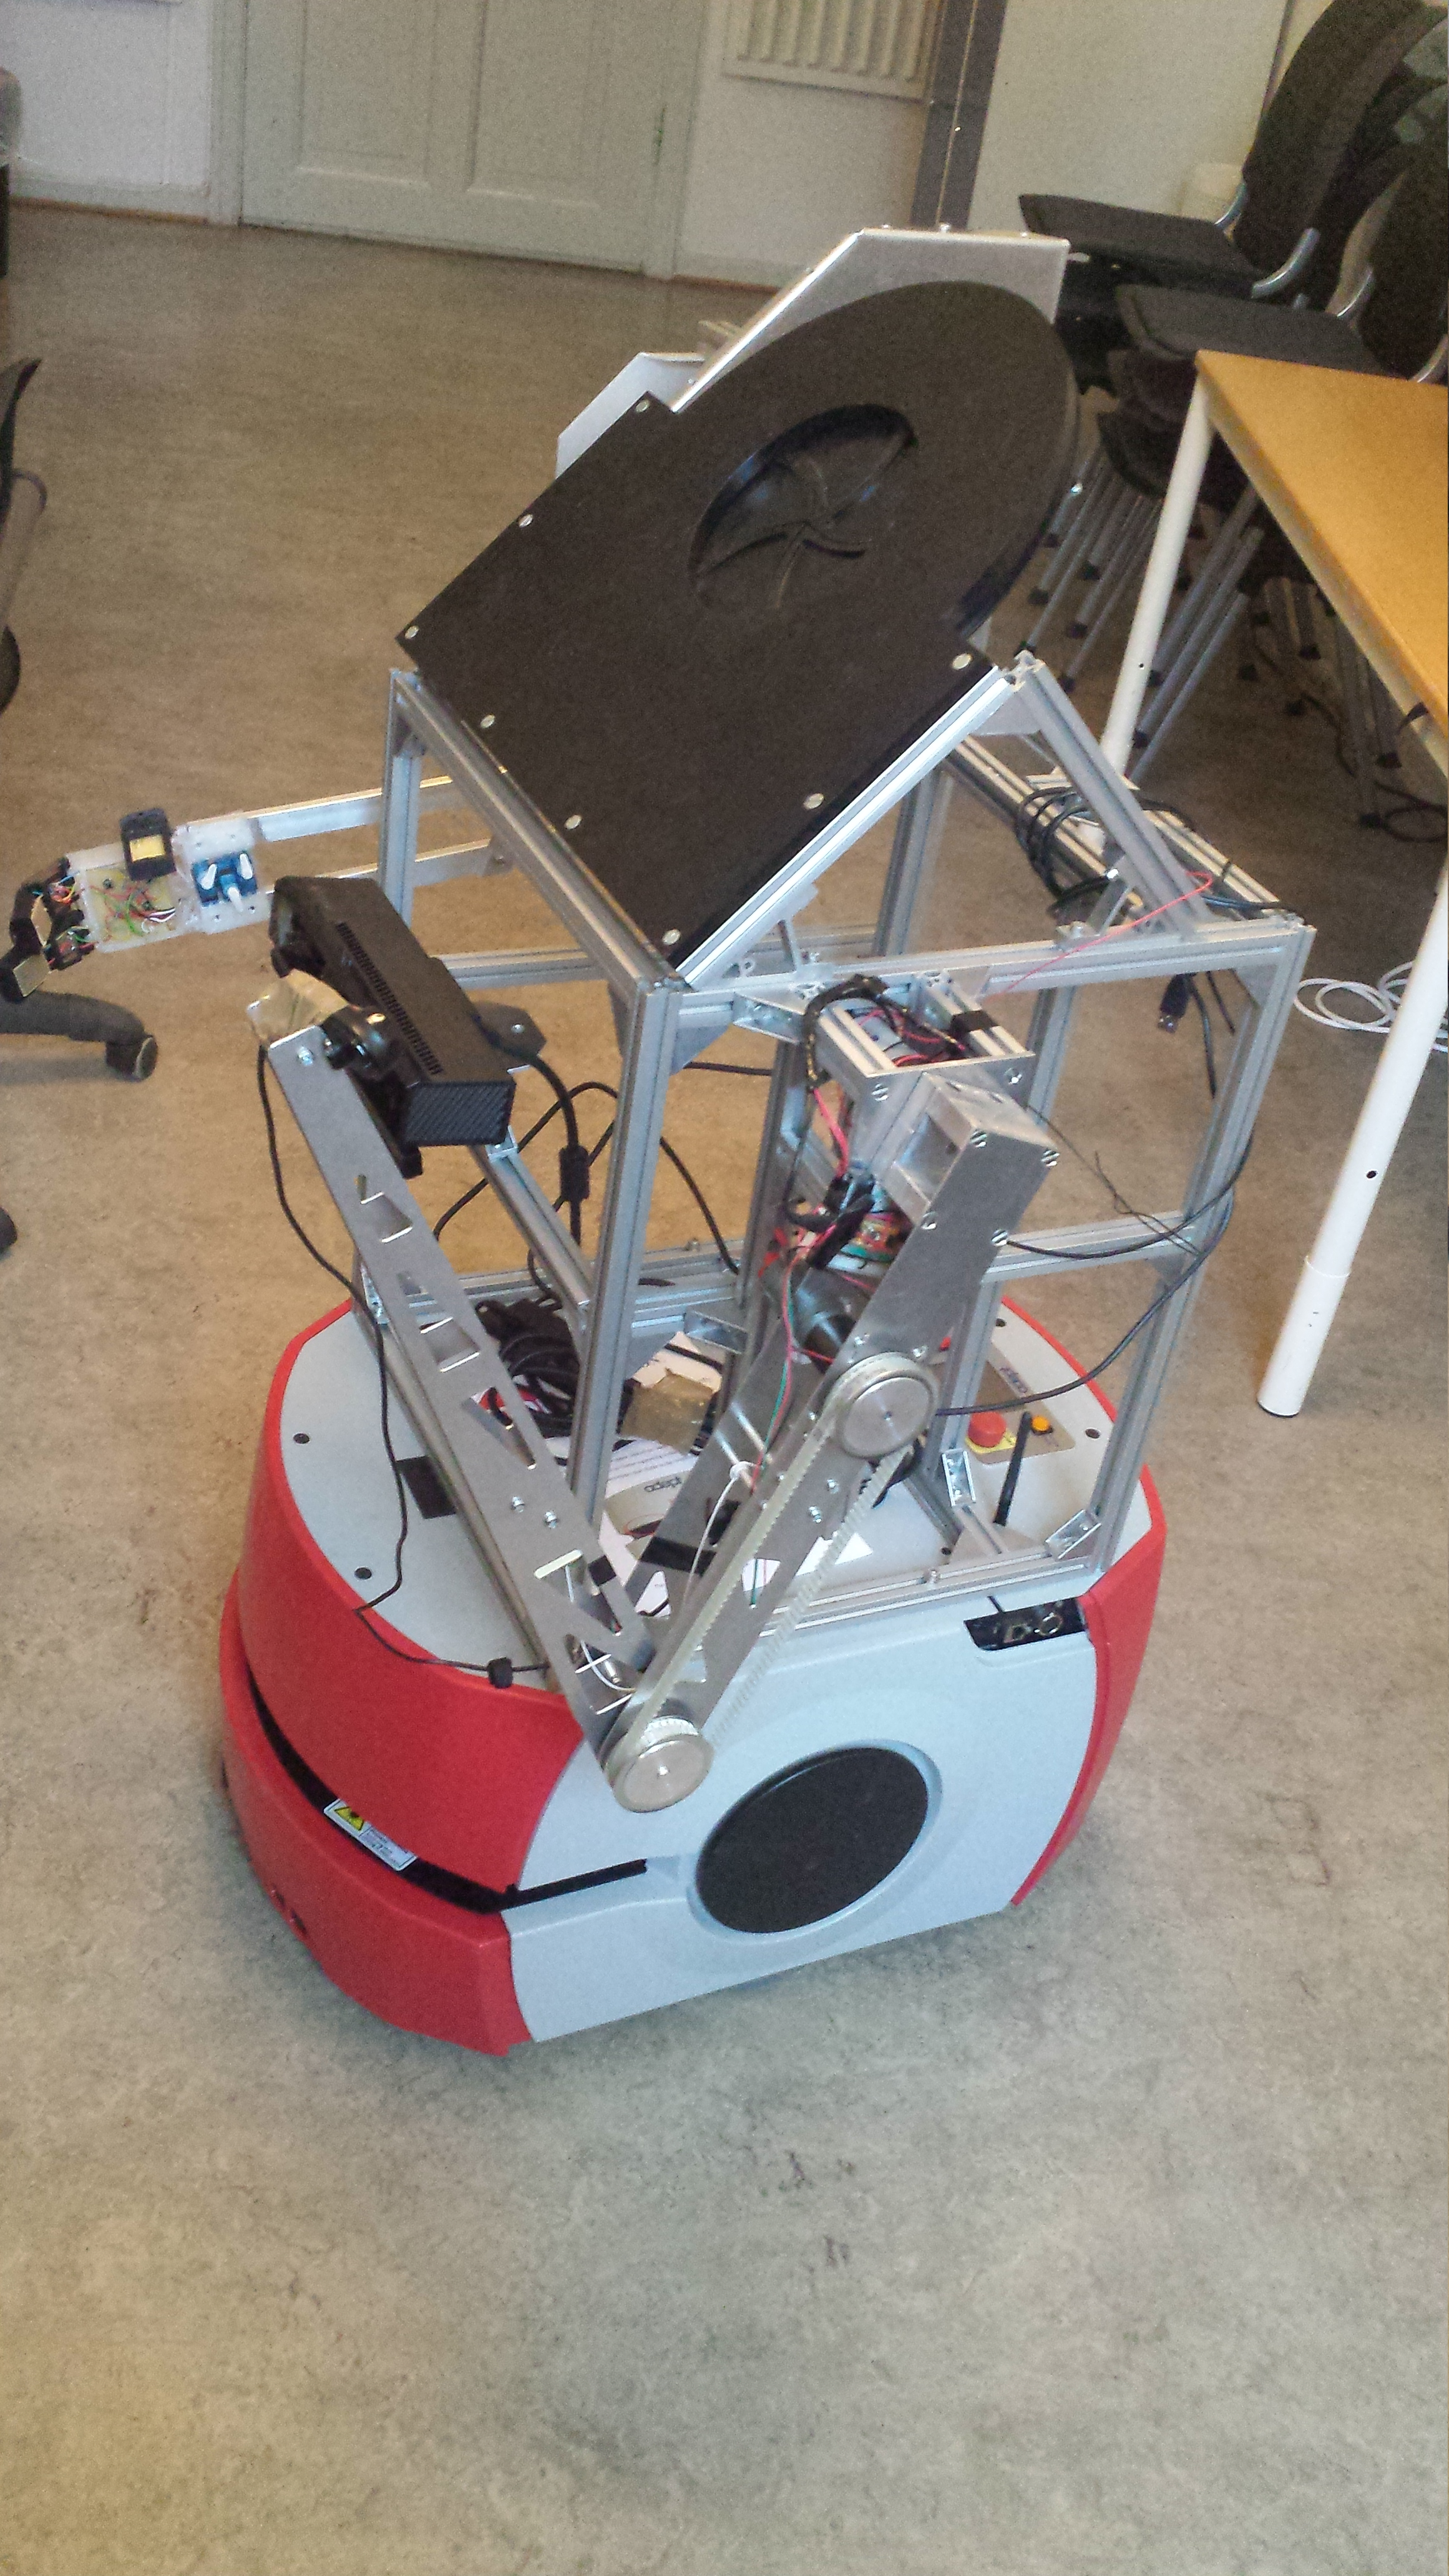
\includegraphics[width=\linewidth]{images/kybrg.jpg}
    \caption{The NTNU cyborg}
    \label{fig:cyborg}
\end{figure}
\subsection{Growing Neurons In Vitro}
The neuron cultures used in the cyborg are being grown in MEAs
at the department of neuroscience.
The MEAs are seeded with neural stem cells of either human or rat origin which
then spontaneously form networks.
At seeding there is no network at all, only a ``soup'' of dissociated neurons
which over the course of several weeks start forming networks.
As the networks starts ``maturing'' a common phenomenon is neurons firing
monotonic spikes automatically.
The activity from these so-called pacemaker neurons can be seen in \ref{fig:pacemaker}.
In the figure each cell corresponds to one of the electrodes as seen in
\ref{fig:cellular_networks}, however at this stage the monotonic spiking
activity tends to be transient, starting and stopping randomly.
\subsection{Neuron Interfacing Hardware}
The hardware used to interface with neuron cultures for the cyborg is an
\textit{MEA2100} system purchased from multichannel systems. 
The MEA2100 system is built to conduct in-vitro experiments electrically active
cell cultures such as neurons.
The principal components of the MEA2100 systems are:
\subsubsection{Micro Electrode Array}
Introduced in the previous chapter, the \textit{MEA} is equipped with an array
of microscopic electrodes capable of sensing and delivering voltages to and from
nearby neurons.
\ref{fig:generic_MEA} shows an empty MEA,
\ref{st_olav_MEA} shows an MEA from st.olavs with a live neuron culture.
\subsubsection{Headstage}
The electrodes of the MEAs are measured and stimulated by the headstage which
contains the necessary high precision electronics needed for microvolt range readings.
\ref{fig:headstage} shows the same type of headstage used in this paper along
with an MEA.
\subsubsection{Interface board}
The interface board connects to up to two head-stages and is responsible for interfacing
with the data acquisition computer, as well as auxiliary equipment such as temperature
controls.
The interface board has two modes of operation.
In the first mode the interface board processes and filters data from up to two
headstages as shown in \ref{fig:IFB_regular} which can then be acquired on a normal
computer connected via USB.
In the second mode of operation a Texas instruments TMS320C6454 digital signal
processor is activated which can then be interfaced with using the secondary USB
port as shown in \ref{fig:IFB_BSP}
\begin{figure}[h!]
    %\centering
    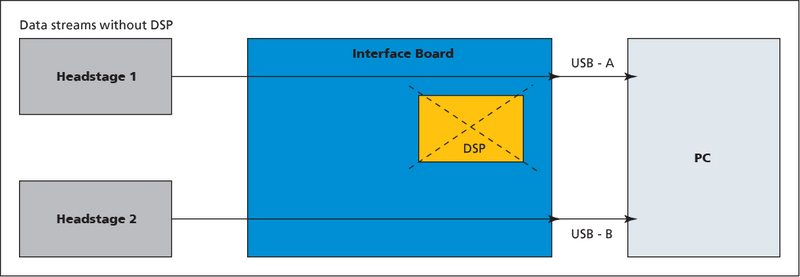
\includegraphics[width=\linewidth]{images/regular_operation.png}
    \caption{Casual mode}
    \label{fig:IFB_regular}
\end{figure}
\begin{figure}[h!]
    %\centering
    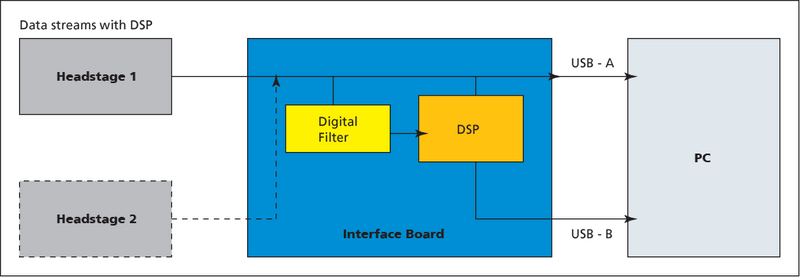
\includegraphics[width=\linewidth]{images/dsp_operation.png}
    \caption{DSP active}
    \label{fig:IFB_DSP}
\end{figure}
\begin{figure}[h!]
    %\centering
    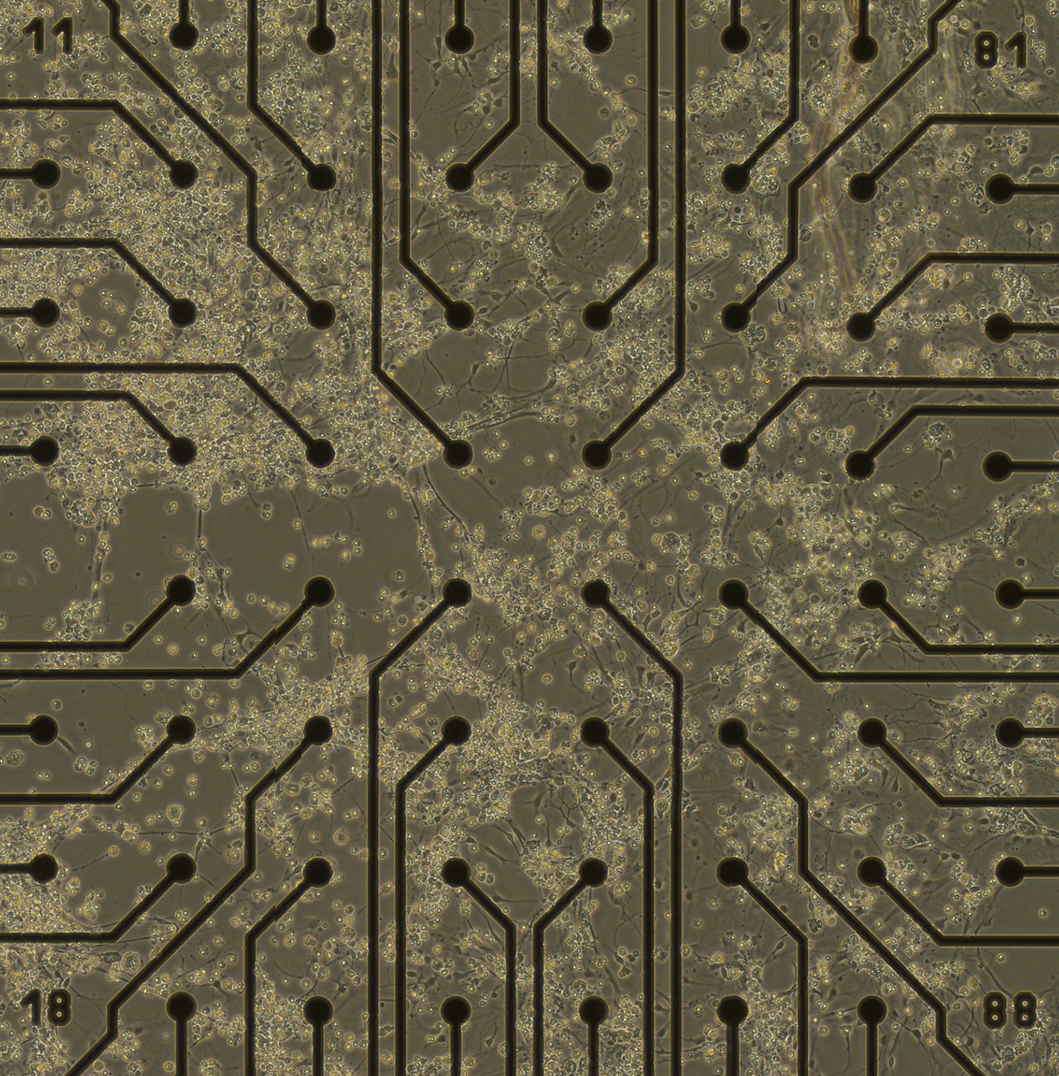
\includegraphics[width=\linewidth]{images/cells.png}
    \caption{Microscopic image on neural networks with visible structures}
    \label{fig:cellular_networks}
\end{figure}
\begin{figure}[h!]
    %\centering
    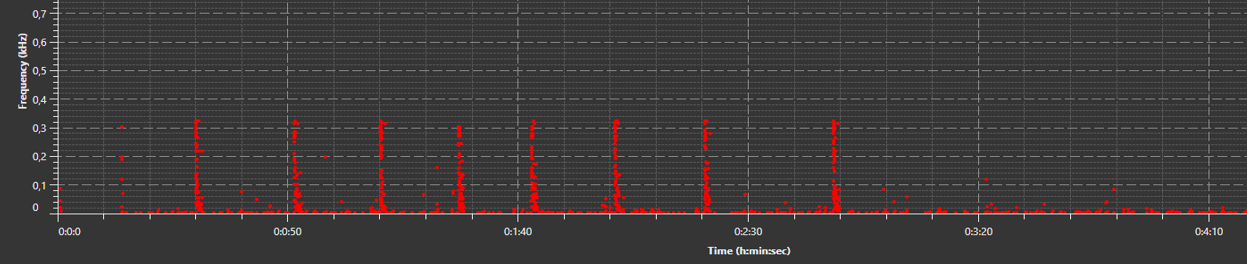
\includegraphics[width=\linewidth]{images/crop_corr28.png}
    \caption{A recording of spikes in a neural culture. Readings performed by
      Ola Huse Ramstad at the department of neuroscience}
    \label{fig:pacemaker}
\end{figure}
\begin{figure}[h!]
    %\centering
    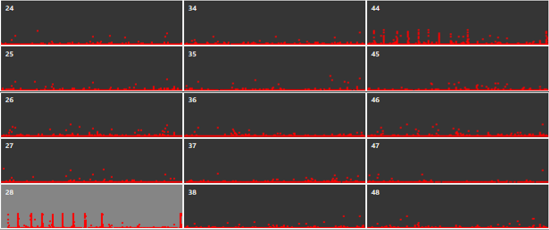
\includegraphics[width=\linewidth]{images/tonic1.png}
    \caption{The grayed out cell in the bottom left shows the readouts in
      \ref{fig:pacemaker}.
      Each cell corresponds to one of the electrodes as seen in
      \ref{fig:cellular_networks}. Even though electrode 28 and electrode 44 are
      far away from each other there seems to be a clear correlation between these two
    sites.}
    \label{fig:correlation}
\end{figure}
\begin{figure}[h!]
    %\centering
    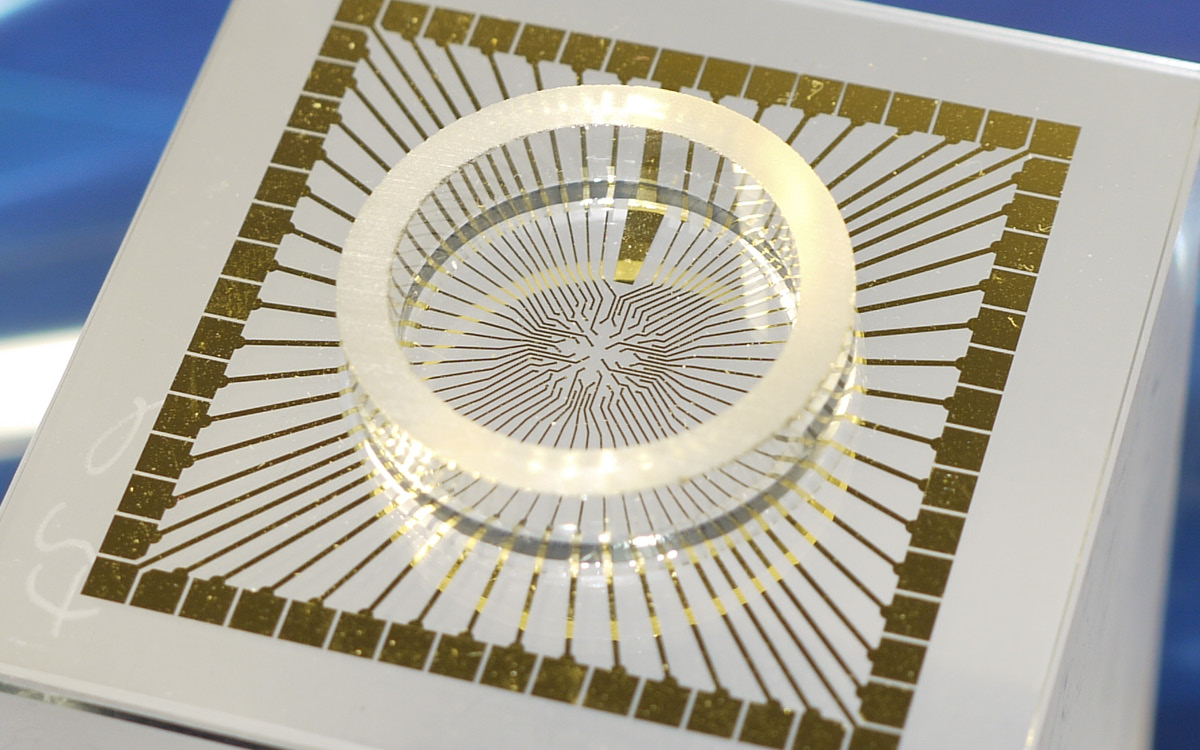
\includegraphics[width=\linewidth]{images/MEA.jpg}
    \caption{A generic MEA}
    \label{fig:generic_MEA}
\end{figure}

\begin{figure}[h!]
    %\centering
    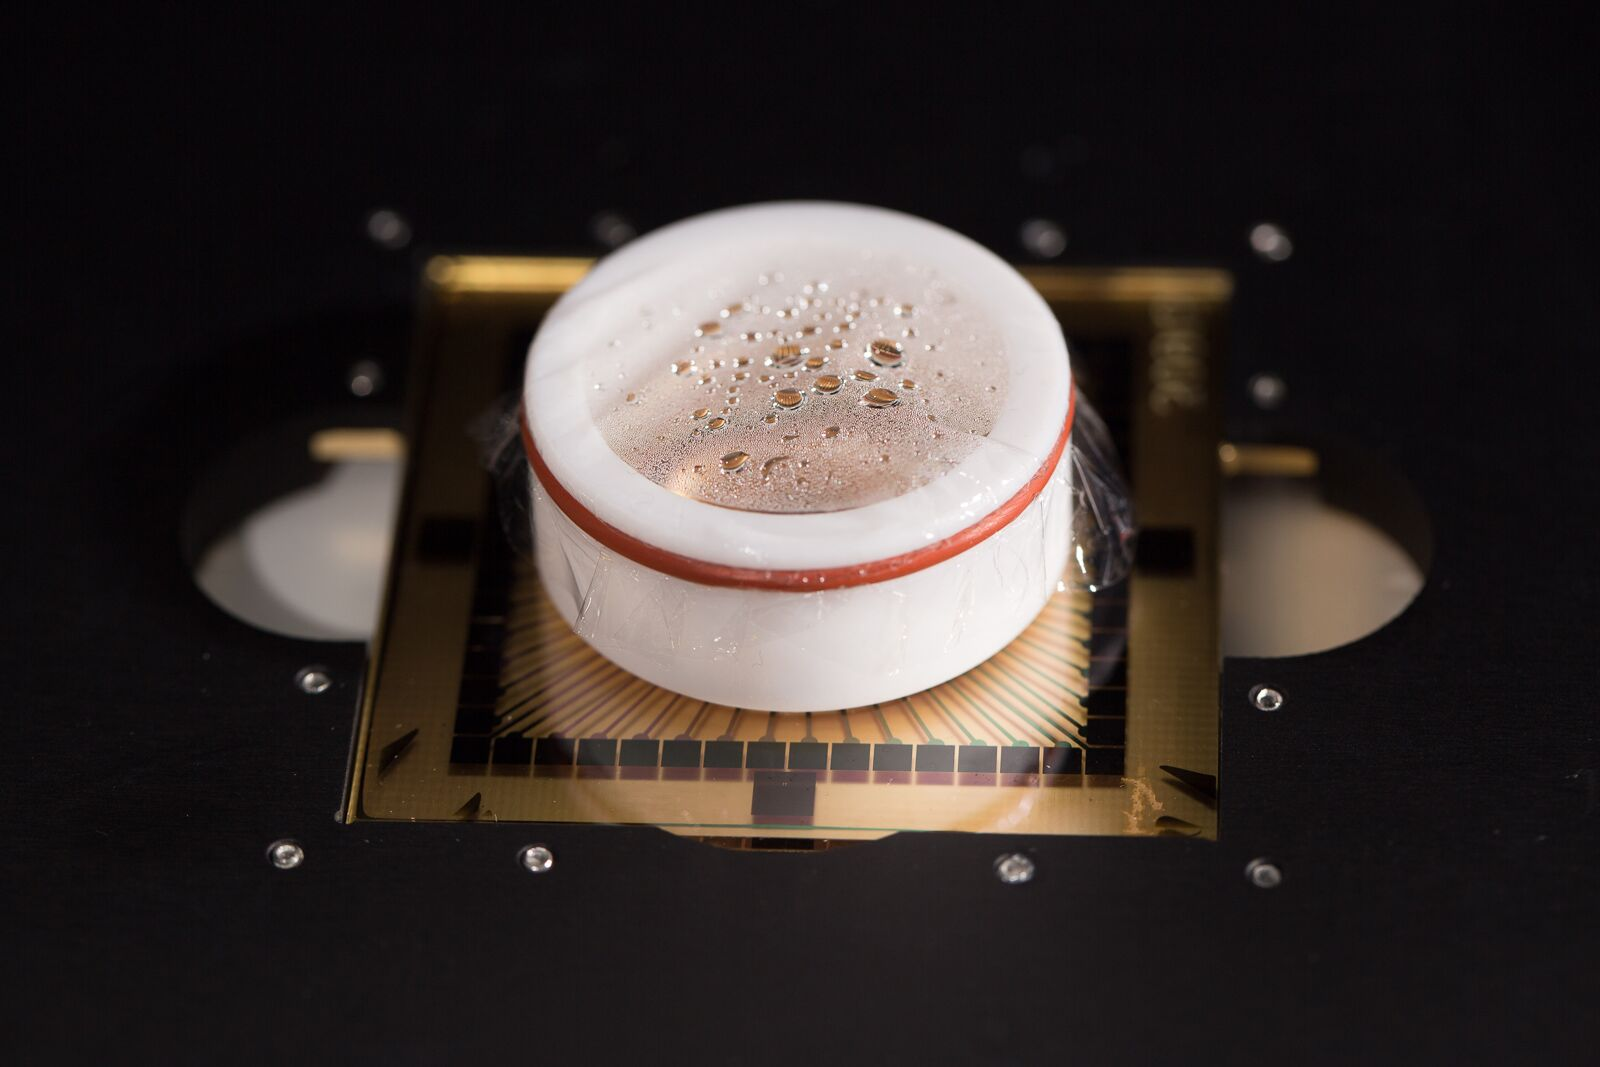
\includegraphics[width=\linewidth]{images/st-olavs-mea.jpg}
    \caption{A MEA with a live culture, photographed by Kai}
    \label{fig:st_olav_MEA}
\end{figure}
\begin{figure}[h!]
    %\centering
    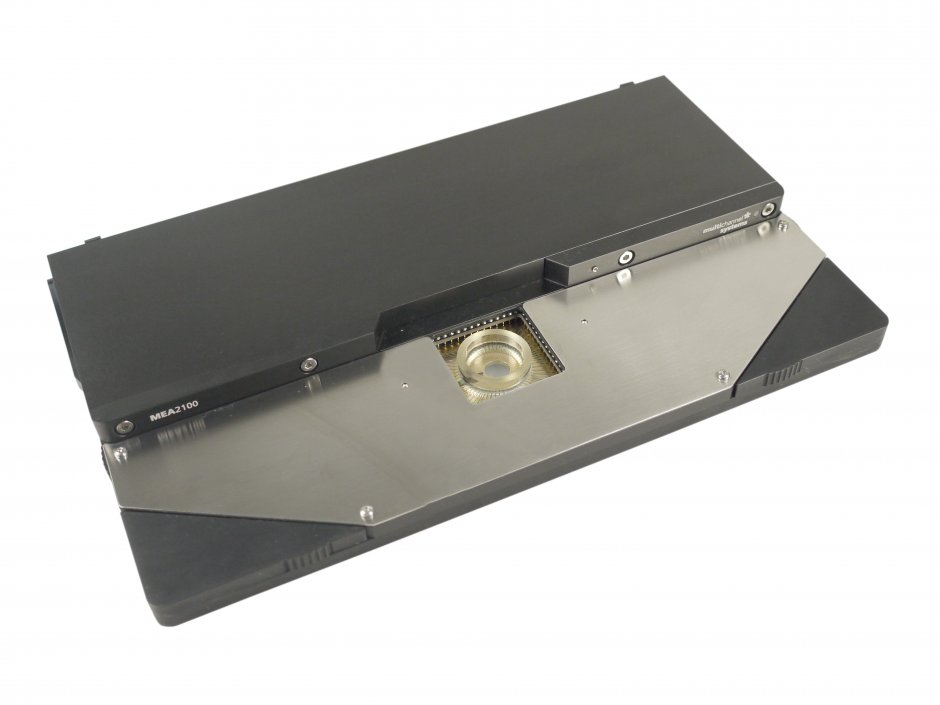
\includegraphics[width=\linewidth]{images/MEA2100-HS60.jpg}
    \caption{The headstage}
    \label{fig:headstage}
\end{figure}
\begin{figure}[h!]
    %\centering
    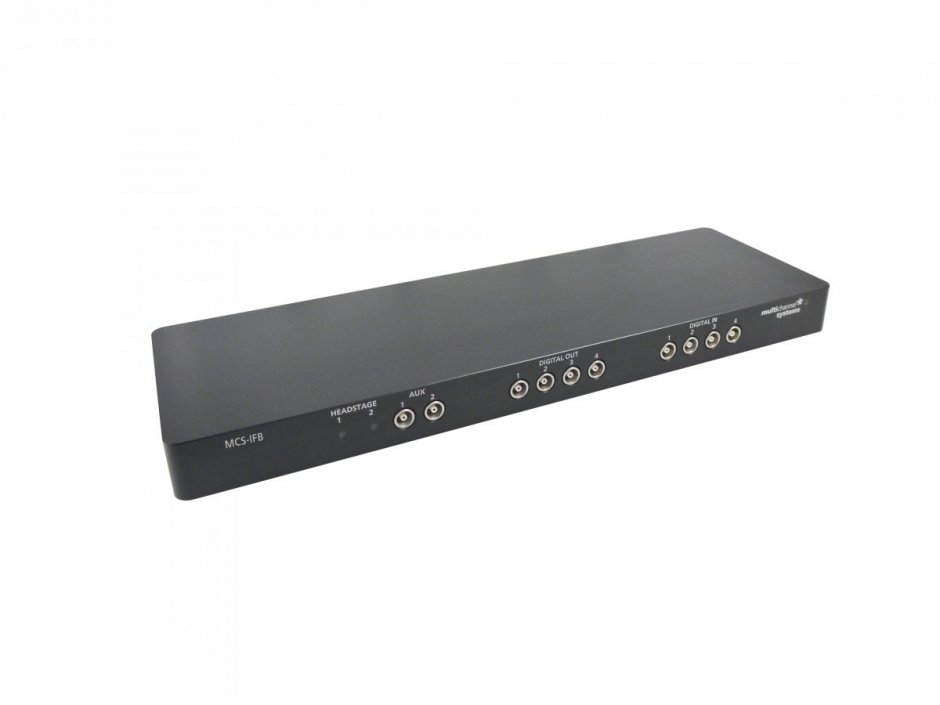
\includegraphics[width=\linewidth]{images/MCS-IFB.jpg}
    \caption{The MCS interface board}
    \label{fig:neuron_anatomy}
\end{figure}
%%% Local Variables:
%%% mode: latex
%%% TeX-master: "../main"
%%% End:

\section{Methodology}
The hardware used to interface with neuron cultures for the cyborg is an
\textit{MEA2100} system purchased from multichannel systems. 
The MEA2100 system is built to conduct in-vitro experiments electrically active
cell cultures such as neurons.
The principal components of the MEA2100 systems are:
\subsubsection{Micro Electrode Array}
Introduced in the previous chapter, the \textit{MEA} is equipped with an array
of microscopic electrodes capable of sensing and delivering voltages to and from
nearby neurons.
\ref{fig:generic_MEA} shows an empty MEA,
\ref{st_olav_MEA} shows an MEA from st.olavs with a live neuron culture.
\subsubsection{Headstage}
The electrodes of the MEAs are measured and stimulated by the headstage which
contains the necessary high precision electronics needed for microvolt range readings.
\ref{fig:headstage} shows the same type of headstage used in this paper along
with an MEA.
\subsubsection{Interface board}
The interface board connects to up to two head-stages and is responsible for interfacing
with the data acquisition computer, as well as auxiliary equipment such as temperature
controls.
The interface board has two modes of operation.
In the first mode the interface board processes and filters data from up to two
headstages as shown in \ref{fig:IFB_regular} which can then be acquired on a normal
computer connected via USB.
In the second mode of operation a Texas instruments TMS320C6454 digital signal
processor is activated which can then be interfaced with using the secondary USB
port as shown in \ref{fig:IFB_BSP}
\begin{figure}[h!]
    %\centering
    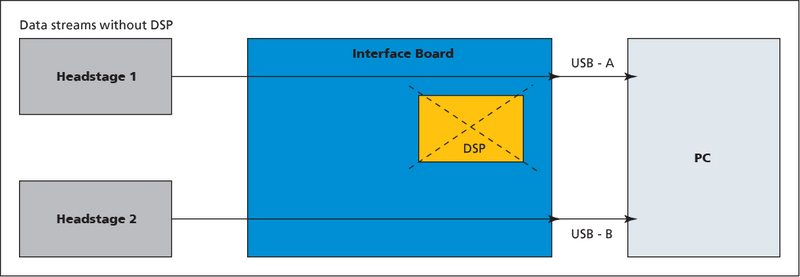
\includegraphics[width=\linewidth]{images/regular_operation.png}
    \caption{Casual mode}
    \label{fig:IFB_regular}
\end{figure}
\begin{figure}[h!]
    %\centering
    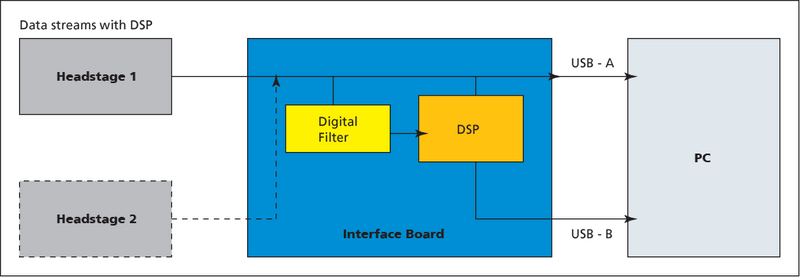
\includegraphics[width=\linewidth]{images/dsp_operation.png}
    \caption{DSP active}
    \label{fig:IFB_DSP}
\end{figure}
%%% Local Variables:
%%% mode: latex
%%% TeX-master: "../main"
%%% End:
\section{Experiments}
In order to show in vitro neuron cultures being viable reservoirs we have
constructed a very simple simulated environment where an agent is placed in a
2D top down environment. The goal of this simulated game is to avoid walls while
exploring (that is, covering ground in order to punish agents that run in
circles or stand still).
In this experiment we wish to show that the neuron reservoir enhances the
performance 
\section{Results}
Describe initial tests running full closed loop system including visualizer bot.
\section{Conclusion}
A working solution for the architectural challenges for interfacing a robot with
a neural cultures has completed a proof of concept test, showing that the remaining
efforts for the cyborg project is harnessing the computations performed by the neural
network.
By proposing the RC cyborg concept as a broader definition of a cyborg the
foundation has been laid for exploring differences between neural networks and other
reservoirs used in the same contextual ``harness'' such that the differences between
reservoirs may be studied quantitatively as well as qualitatively.
With the theoretical and practical framework needed to interface with neural network
the cyborg project is now equipped to explore the fundamental aspects of neural
computation.
\section{Further Work}
\subsection{Exploring Reservoirs}
Only neural networks and random boolean networks have been used as reservoirs.
One of the stated goals of the RC cyborg platform is to facilitate the use of a
wide range of reservoirs ranging from recurrent artificial neural networks, to
more exotic physical reservoirs.
By comparing performance of different reservoirs for the same task different
characteristics impacting performance of RC systems may be explored.
\subsection{Investigating Neuron Growth Rules}
Neural cultures change their own structure in response to stimuli, which in turn
is a result of their structure.
This interplay between self-organization and current dynamics of the neural
network is not well understood, but it may have a profound impact on creating
artificial neural networks imitating their biological counterparts.
One experiment that might shed light on this process is to observe the
differences in regularity between neural networks who have been subjected to
random stimuli compared to cultures who have experienced regular stimuli.
\subsection{Integrating Machine Learning}
In order for SHODAN to support generalized RC tools for machine learning is
required.
A framework for genetic algorithms in scala, named scalapagos, is currently
being implemented and will be used to explore the parameter spaces both for
reservoirs and for data processing reservoir input and output.
%%% Local Variables:
%%% mode: latex
%%% TeX-master: "../main"
%%% End:


\section*{Acknowledgment}
The authors would like to thank...\\
Sandoz, couldn't have done it without you.


\bibliography{mylib} 
\bibliographystyle{ieeetr}

\end{document}
